% The section about the agents' routes
% @author Kalvin Döge
%

\subsection{Agentenrouten}\label{subsec:routs}

In diesem Model haben \code{HumanTraveler} nur zwei Punkte auf ihrer Route, die sie erreichen müssen: Den Startpunkt, auf dem sie beginnen, und das Endziel, das ein beliebiger Punkt im Simulationsbereich ist.
Diese Agenten haben, wie bei dem Unterkapitel ,,Modalitäten`` bereits erwähnt, dafür drei verschiedene Transportarten zur Verfügung, und sind nicht weiter eingeschränkt in der Art und Weise, wie sie zum Zielpunkt gelangen.

\begin{figure}[h]
    \centering
    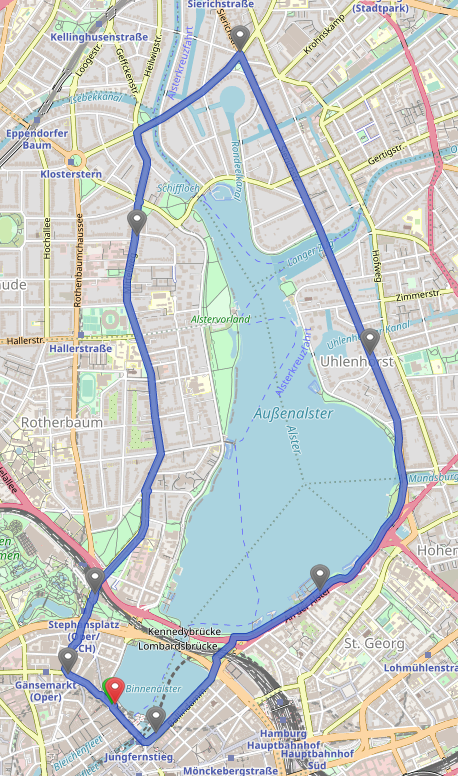
\includegraphics[width=1.00\textwidth]{route}
    \caption{Route der Bicycle-Leader mit den 8 Zwischenpunkten}
    \label{fig:bicycleleader-route}
\end{figure}

Der \code{BicycleLeader} wiederum, wie anhand der Grafik~\ref{fig:bicycleleader-route} zu entnehmen ist, hat 8 Punkte abzufahren, die um die Binnen- und Außenalster verteilt sind:
Die Route beginnt und endet bei dem Café Alex, während die restlichen 6 Punkte verteilt um die Alster platziert sind, damit eine Rundfahrt bei möglichst vielen Lichtsignalschaltungen geplant sind.

